\chapter[Robot Nonverbal Immediacy and Child Learning]{Robot Nonverbal Immediacy and \texorpdfstring{\\}{} Child Learning} \label{chap:nviexperiment} 

\begin{framed}
	\textbf{Key points:}
	
	\begin{itemize}
	\item An experiment is devised to test the effects of high and low \gls{nonverbalimm} behaviours when applied to robot social behaviour.
	\item The methodology builds on the one used in the last chapter: teaching children how to identify prime numbers. The robot behaviour in this chapter is derived from principles of \gls{nonverbalimm}, rather than from a human model. This allows for a stronger theoretical underpinning in terms of what constitutes social behaviour, and provides a directly measurable manipulation of robot behaviour.
	\item Children learn a significant amount from a robot perceived by the children as having higher \gls{nonverbalimm}, but do not undergo significant \gls{learning} with a lower \gls{nonverbalimm} robot.
	\item These findings confirm predictions from the human-human \gls{immediacy} literature and provide a basis for robot social behaviour implementation in educational interactions.
	\end{itemize}
\end{framed}

Part of the work presented in this chapter has been published in \cite{kennedy2015higher}. The final publication is available from Springer via:\newline http://dx.doi.org/10.1007/978-3-319-25554-5\_33

\newpage
Chapter~\ref{chap:embodiment} demonstrated the social advantages that using a physically present social robot can bring to interactions with children. These findings were furthered in Chapter~\ref{chap:socasoc} where children learnt a significant amount from a social robot and touchscreen, but did not experience such \gls{learning} gains when provided with the same information on a touchscreen alone. However, Chapter~\ref{chap:socasoc} also revealed surprising \gls{learning} results in response to different robot social behaviours. These behaviours were based on a human model completing the same task, and an `inverse' set devised by the author. These behaviours were intended to provide maximal differences between conditions to demonstrate the positive effect of appropriate social behaviour. However, the results were not as expected, with the inverse set of behaviours (expected to be inappropriate for inducing \gls{learning}) instead leading to significant \gls{learning}.

This chapter seeks to further explore the impact of robot social behaviour on child \gls{learning}. The lesson content from the previous chapter is maintained, but the robot behaviour used here is different. The aim is to remove any confounds relating to the personalisation contained in the behaviour of the previous chapter (these personalisations were part of the human model and were not distinctly separable from the general social behaviour). In order to do this, the social behaviour derived from the human model is substituted for behaviour derived from the principles of \gls{nonverbalimm} as described in the literature and specified in the \gls{nonverbalimm} scale \citep{richmond1998nonverbal}.

%%%%%%%%%%%%%%%%%%%%%%%%%%%%%%%%%%%%%%%%%%%%%%%%%%%%%%%%%%%
\section{Hypotheses} \label{sec:meth-hyp}
The \acrshort{hhi} literature has shown that greater instructor \acrshort{nvi} leads to increased cognitive \gls{learning} gains \citep{witt2004meta}. These findings have been partially confirmed in \acrshort{hri} \citep{szafir2012pay}, but using only 2 modalities (speech and gesture). Nonetheless, survey data showed that participants could perceive such behavioural differences. Previous work in Chapter \ref{chap:socasoc} conducted in a similar context to this study found that children gazed more at a `more social' robot tutor during lessons, and were more likely to report it to be like a friend than an equally active, but counter-social, robot tutor. It could be argued that an increase in \acrshort{nvi} behaviour is analogous to an increase in social skills, so the same perceptual and behavioural differences of children could be predicted here, leading to H2 and H3. Based on these prior findings, the following hypotheses were devised:

\begin{enumerate}
\item [\textbf{H1}:] A robot with higher \gls{nonverbalimm} will lead to greater child cognitive \gls{learning} gains.
\item [\textbf{H2}:] Children will regard a robot with high \gls{nonverbalimm} more like a friend than one with low \gls{nonverbalimm}.
\item [\textbf{H3}:] Children will gaze at a robot with high \gls{nonverbalimm} more during the prime lesson period than at a robot with low \gls{nonverbalimm}.
\end{enumerate}

%%%%%%%%%%%%%%%%%%%%%%%%%%%%%%%%%%%%%%%%%%%%%%%%%%%%%%%%%%%
\section{Experimental Setup}\label{sec:nviprimes-setup}
The study here uses 2 conditions in a between-subjects design, both using a robot, with the nonverbal immediacy manipulated to create contrasting robot social behaviours. The methodology used in this study is as established in prior studies and Chapter~\ref{chap:method}. A robot is used as a tutor in one-to-one interactions to teach children how to identify prime numbers between 10 and 100 based on whether they are divisible by 2, 3, 5 or 7. The children participating in the interactions do not have prior knowledge of prime numbers, but have the skills to do the division (albeit with imperfect performance), making the combination of these skills into a rule for categorising primes possible in a short interaction. Prior knowledge is assessed with a pre-test. The novel difference between the present study and previous work is in the robot behaviour. Previously the social behaviour was based on a human model, whereas in this study the robot behaviour is derived from \acrshort{nvi} concepts (detailed in Chapter~\ref{chap:background}).

\subsection{Participants} \label{sec:meth-participants}
The study was conducted in a class of children aged 8-9 years old. All children interacted with the robot, but due to breaks in protocol, and one statistical outlier (Grubbs' test), several interactions were excluded from the analysis. A total of 23 interactions were considered (16F/7M, age \textit{M}=8.74, \textit{SD}=0.45). All subjects had permission from a parent/guardian to participate in the study. Of the 23 subjects, 21 also had permission to be filmed for video analysis.

\subsection{Interaction Protocol} \label{sec:meth-intstruct}
Interactions took place in an empty room familiar to the children near to their classroom. The children were briefed by one of the experimenters before entering the room. Two experimenters were present in the room, out of view of the child whilst they interacted with the robot. The child sat across a large touchscreen from an Aldebaran NAO robot (Figures~\ref{fig:ch8_highsnap} and \ref{fig:ch8_lowsnap}). A Microsoft Kinect was placed behind the robot to track the child's head gaze. Video cameras were placed behind the robot and behind the child to record the interaction. The average time spent interacting with the robot was \textit{M}=14m19s, \textit{SD}=3m27s. The average interaction time from the videos (from entering the experiment room, to exiting -- therefore including questionnaire time) was \textit{M}=19m19s, \textit{SD}=3m43s.

\begin{figure}[t!]
    \centering
    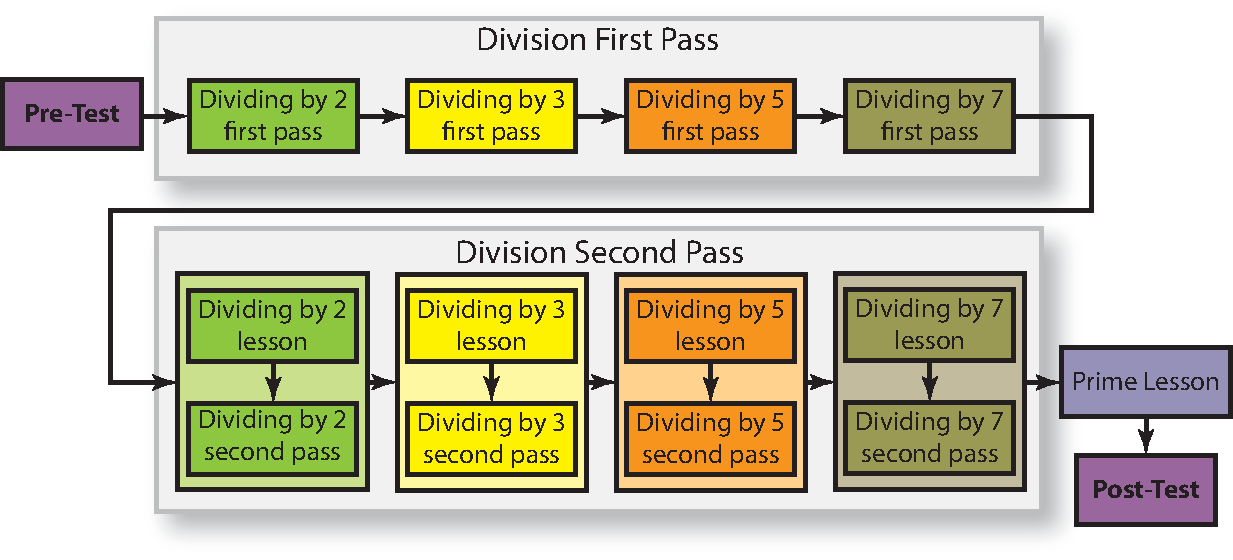
\includegraphics[width=1.0\textwidth]{images/ch7_task_structure.pdf}
    \caption{Structure of the task used in the interactions, showing robot lesson positions (identical to Chapter~\ref{chap:socasoc} Figure~\ref{fig:ch7_structure}).}
    \label{fig:ch8_structure}
\end{figure}

\begin{figure}[t!]
    \centering
	 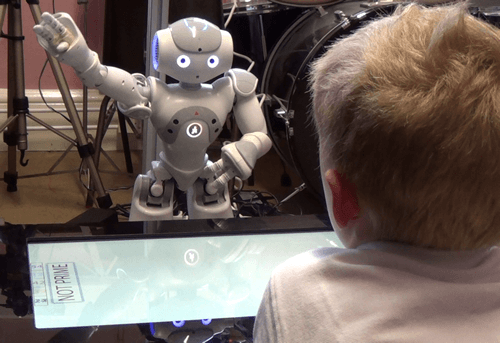
\includegraphics[width=0.7\textwidth]{images/ch8_still_IM_comp.png}
    \caption{A snapshot from the `high' nonverbal immediacy condition.}
    \label{fig:ch8_highsnap}
\end{figure}

\begin{figure}[t!]
    \centering
	 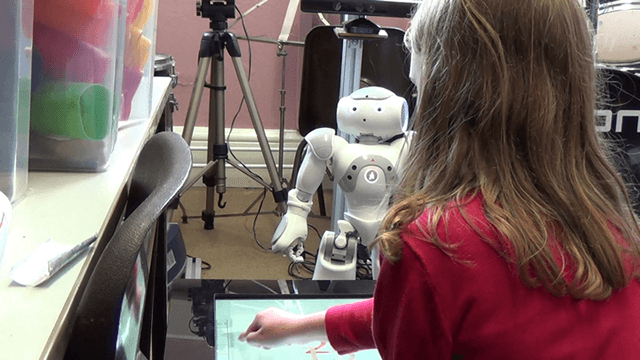
\includegraphics[width=0.7\textwidth]{images/ch8_still_NI_comp.png}
    \caption{A snapshot from the `low' nonverbal immediacy condition.}
    \label{fig:ch8_lowsnap}
\end{figure}

The robot would first introduce itself and ask the children to complete a pre-test on the touchscreen for prime numbers, and then pre-tests for each of the divisors (2, 3, 5 and 7). The robot would then deliver a lesson for each of the divisors and ask the child to complete a post-test following this lesson, i.e., the robot gives a lesson on dividing by 2 and then the child does a dividing by 2 post-test, followed by dividing by 3 lesson and post-test, and so on. After this had been completed, the robot delivered a lesson about prime numbers which combined the lessons for the divisors into a rule for determining whether a number between 10 and 100 is prime (a variation on the \textit{Sieve of Eratosthenes} method). The interaction with the robot would finish with a prime number post-test.

The prime number pre- and post-tests both consist of 12 numbers which must be categorised as `prime' or `not prime'. Two sets of numbers were used for these tests, which are alternately used as the pre- and post-tests in a cross testing strategy to control for potential difference in test difficulty. The tests were balanced in terms of the number size, as it was assumed that higher numbers would be harder for the children to work with. The divisor pre-tests consist of 8 numbers which must be categorised as either `can divide by \textit{X}', or `can't divide by \textit{X}' (where \textit{X} is 2, 3, 5 or 7, Figure~\ref{fig:ch8_structure}). The divisor post-tests are the same, but with 6 numbers instead of 8. In all pre- and post-tests, an equal quantity of numbers belong to each category.

After the interaction with the robot is finished, the child is asked by the experimenter to complete two questionnaires. The first questionnaire was a Robot Nonverbal Immediacy Quesionnaire (RNIQ), adapted from the short-form \acrshort{nvi} questionnaire \citep{richmond1998nonverbal}, described in Chapter~\ref{chap:method} and available in Appendix \ref{app:rniq}. The second questionnaire consisted of two multiple choice questions, asking the children what they thought the robot was like (8 options including friend and teacher), and what they thought playing with the robot was like (4 options, plus a free text box) -- available in Appendix~\ref{app:rrq}.

\subsection{Robot Behaviour} \label{sec:meth-robotbehave}
The robot social behaviour was generated by considering the \acrshort{nvi} questionnaire measures, as seen in \citet{richmond2003development}. The intention was to create high and low \acrshort{nvi} conditions in order to address the hypotheses for the study (Section~\ref{sec:meth-hyp}). Each of the modalities rated in the RNIQ was considered for the Aldebaran NAO robot. Some of the modalities are not possible to manipulate (for example the NAO cannot perform facial expressions), but the other modalities were considered in turn and designed to be either maximally or minimally immediate. Table~\ref{tab:rob-conditions} shows the differences between the two robot conditions. All robot behaviour was autonomous, a `Wizard-of-Oz' was only employed to click a button to begin the behaviour once the child was in position in front of the robot/screen.

Children were assigned to conditions randomly, whilst balancing for gender and mathematical ability (as judged by the class teacher). This led to 12 children in the low \acrshort{nvi} condition (9F, 3M) and 11 children in the high \acrshort{nvi} condition (7F, 4M) after exclusions.

\begin{table}[t!]
	\centering
	\renewcommand{\arraystretch}{1.2} 
	\begin{tabular}{@{}ll@{}}
	\toprule
	\textbf{High Nonverbal Immediacy}	& \textbf{Low Nonverbal Immediacy} 	\\ \midrule
	Leans forwards										& Leans backwards 									\\
	\begin{tabular}[c]{@{}l@{}}Actively gazes at child\\ (with frequent movement)\end{tabular} & \begin{tabular}[c]{@{}l@{}}Looks up and away from child\\ (with occasional movement)\end{tabular} 		\\
	Frequent gestures while talking          & No gestures while talking 						\\
	Standard TTS                                           & TTS modified to make voice ``dull''      \\
	\begin{tabular}[c]{@{}l@{}}Continuous small upper body \\ movements (relaxed upper body)\end{tabular} & Rigid/tense upper body with no movement          																							\\ \midrule                                               
	\end{tabular}
	\caption{Robot behaviour for high and low nonverbal immediacy (\acrshort{nvi}) conditions.}
	\label{tab:rob-conditions}
\end{table}

%%%%%%%%%%%%%%%%%%%%%%%%%%%%%%%%%%%%%%%%%%%%%%%%%%%%%%%%%%%
\section{Results}\label{sec:nviprimes-results}
\subsection{Learning Gains}
To test the impact of the robot's lessons on the children's division skills, the percentage score of division across all pre-tests was compared with the score across all division post-tests. The two pre- and post-test groups were compared with independence of observations (as there were a different number of items in the pre- and post-tests), and a continuous measure. Distributions did not significantly deviate from normality (Kolmogorov-Smirnov test; $\textit{p}>.05$) and had homogeneity of variances (Levene's test; $\textit{p}>.05$). For this reason, a two-tailed independent samples \textit{t}-test is used. A significant difference is found between the division pre-test percentage (\textit{M}=0.84, 95\% CI [0.80,0.88]) and the post-test percentage (\textit{M}=0.89, 95\% CI [0.85,0.92]); \textit{t}(22)=2.081, \textit{p}=.049. This demonstrates that the children can learn from the robot and suggests that the lessons that the robot delivers are appropriate.

All scores for the prime number pre- and post-tests are out of 12. Given that the children have no prior knowledge of prime numbers and there are 2 potential categories for each image, a pre-test score of 6 (50\%) would be expected from random behaviour. Two groups (pre-test and post-test) are compared with paired values on a continuous measure, distributions did not significantly deviate from normality (Kolmogorov-Smirnov test; $\textit{p}>.05$). As such, a paired samples \textit{t}-test is used. In the low \acrshort{nvi} condition the improvement from pre-test (\textit{M}=7.08, 95\% CI [5.01,9.15]) to post-test (\textit{M}=8.00, 95\% CI [6.24,9.76]) is not statistically significant; \textit{t}(11)=0.754, \textit{p}=.466. However, in the high \acrshort{nvi} condition the difference from pre-test (\textit{M}=5.09, 95\% CI [3.43,6.75]) to post-test (\textit{M}=7.00, 95\% CI [4.88,9.12]) is statistically significant at the \textit{p}\textless .05 level; \textit{t}(10)=3.057, \textit{p}=.012 (Figure~\ref{fig:ch8_graphs}).

The pre-test score appears to be very different between the conditions, however this was not found to be significant; \textit{t}(21)=1.640, \textit{p}=.116. The 95\% confidence interval for the pre-test in both conditions covers the expected value of 6, which reassures that the children did not know what primes were before the intervention. Additionally, there is no significant difference between the two different pre-test scores, or of the improvement between pre- and post-test, regardless of which of the two pre-tests were taken; this shows that the tests can be considered of equal difficulty. Therefore, support has been shown for Hypothesis~1: children interacting with the high \acrshort{nvi} robot benefit from increased cognitive \gls{learning} gains. However, this is slightly tempered, as there is no significant difference between conditions. Children in both conditions are likely to improve (which isn't surprising given practice and teaching input), but those in the high \acrshort{nvi} condition undergo significant improvement, whereas those in the low immediacy condition do not.

\begin{figure}[t!]
    \centering
    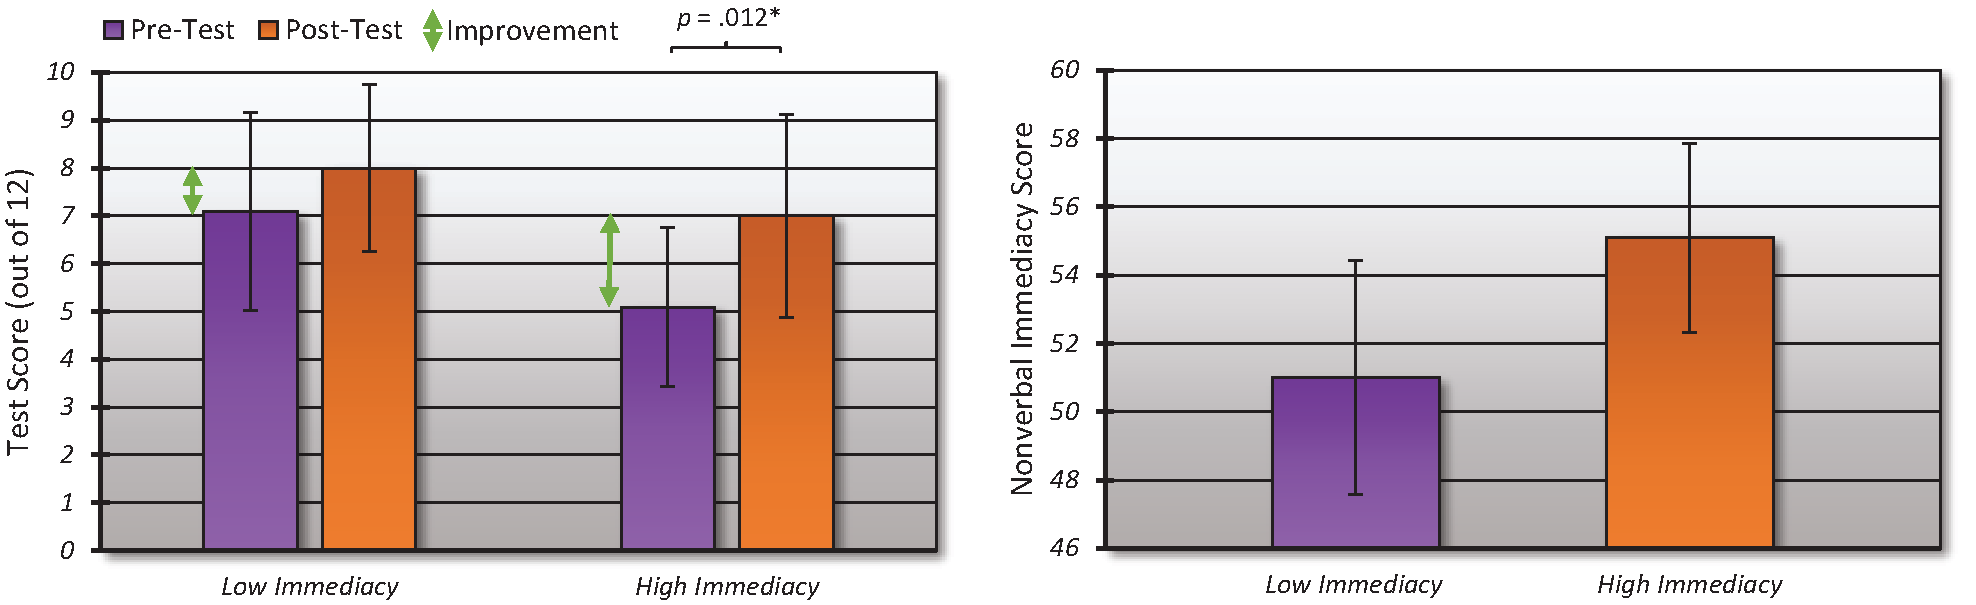
\includegraphics[width=1.0\textwidth]{images/ch8_graphs.pdf}
    \caption{Pre- and post-test scores on recognising prime numbers for the low and high \gls{nonverbalimm} (\acrshort{nvi}) conditions (\textit{left}); \acrshort{nvi} scores for the designed low and high \acrshort{nvi} conditions (\textit{right}). Children improve more in recognising prime numbers when taught by a high immediacy robot. \textit{Error bars} show 95\% CI.}
    \label{fig:ch8_graphs}
\end{figure}

\subsection{Questionnaire Data}
After the children had interacted with the robot they were asked to complete the \acrshort{rniq} on paper. Immediacy scores are calculated from the answers to the \acrshort{rniq} questions: the higher the resulting number, the higher the perceived immediacy. The score can be up to 80, but there are a number of measures for which there are no equivalent robot behaviours (e.g., touching the child). Therefore, a score of around 56 would indicate a rating of near-maximal \acrshort{nvi} given the modalities which are manipulated. This reduction in the expected score also inhibits the potential for difference between conditions, as for many of the questionnaire elements, the behaviour is the same (e.g., the lack of facial expressions).

The designed low immediacy condition received a mean \acrshort{nvi} score of \textit{M}=51.0 (95\% CI [47.6,54.4]). The designed high immediacy condition received a mean score of \textit{M}=55.1 (95\% CI [52.3.57.9]). An unpaired \textit{t}-test is used as these groups are independent observations. The test reveals that this difference falls just outside of significance at the \textit{p}\textless .05 level; \textit{t}(21)=2.031, \textit{p}=.055 (Figure~\ref{fig:ch8_graphs}). However, the subject numbers are relatively low and if the trends seen were to continue, then this difference would become significant. Indeed, the differences between the means only just includes no difference; $-0.10 \leq \mu _{HNVI} - \mu _{LNVI} \leq 8.28$. This provides reasonable support for the manipulation check; children perceive a robot designed to be more nonverbally immediate as such.

The second questionnaire that the children completed asked them what the robot was like, and what playing with the robot was like. The children were asked ``For me, I think the robot was like a -'', and had 8 options to choose from (brother or sister, classmate, stranger, relative (e.g., cousin or aunt), friend, parent, teacher, neighbour). Given Hypothesis~2 (that children in the high immediacy condition will more frequently report the robot to be like a friend) the responses were sorted into whether the children responded that the robot was like a friend, or not. In the high immediacy condition 6 children reported the robot to be like a friend and 5 not (with all selecting `teacher'), whereas in the low immediacy condition 1 child reported the robot to be like a friend and 11 not (1 `classmate', 10 `teacher'). Fisher's exact test reveals a significant difference between the conditions, with those in the high immediacy condition significantly more likely to report that the robot is like a friend than those in the low immediacy condition; \textit{p}=.027. Therefore Hypothesis 2 is supported.

This result is surprising as the children are told multiple times by both the experimenter and the robot that the robot is a \textit{teacher robot} which will teach them some maths. However, the same result has previously been found, which led to the formulation of Hypothesis 2: children interacting with a `more social' robot reported more frequently that the robot is like a friend (as in the previous chapter; published in \citealp{kennedy2015robot}).

\subsection{Gaze Analysis}
The 21 videos from the interactions were manually coded for child gaze during the prime lesson segment as this has previously been found to be indicative of overall gaze patterns in the interaction (Chapter~\ref{chap:socasoc}, and the prime lesson constitutes a key part of the interaction in terms of the \gls{learning} outcome. One of the 21 videos was excluded due to occlusions, leaving 9 videos from the high immediacy condition and 11 from the low. 20\% of the remaining videos were second coded to verify validity, with a mean Cohen's Kappa of 0.83, indicating \textit{almost perfect} agreement.

No significant difference was found between the length of time children gaze at the robot in seconds per minute of the prime lesson segment between the high \acrshort{nvi} condition (\textit{M}=15.9, 95\% CI [11.3,20.5]) and the low \acrshort{nvi} condition (\textit{M}=15.4, 95\% CI [11.9,18.6]); \textit{t}(18)=0.214, \textit{p}=.832. Nor is there a significant difference in the number of times children gaze at the robot per minute of the prime lesson segment between the high \acrshort{nvi} condition (\textit{M}=15.2, 95\% CI [12.2,18.2]) and the low \acrshort{nvi} condition (\textit{M}=14.7, 95\% CI [11.7,17.7]); \textit{t}(18)=0.234, \textit{p}=.817. Therefore, Hypothesis 3 (children will gaze more at the high \acrshort{nvi} robot) is not supported. This is a surprising result, which possibly strengthens the link between robot behaviour and \gls{learning}. If gaze is considered to be a reflection of child attention, then despite equivalent attention during the key piece of \gls{learning} input from the robot the \gls{learning} results still vary, suggesting that the robot social behaviour could be responsible. Of course, this is just one of many possibilities and the gaze could be equal simply because the behaviour during this phase is quite novel compared to the rest of the interaction.

%%%%%%%%%%%%%%%%%%%%%%%%%%%%%%%%%%%%%%%%%%%%%%%%%%%%%%%%%%%
\section{Discussion}\label{sec:nviprimes-discussion}
The manipulation check revealed that children do recognise when a robot has higher or lower \gls{nonverbalimm}. The difference was close to significance at the 5\% level, with the difference between the means only just including no difference. This finding shows that the robot behaviour is largely interpreted by the children as intended by the designer, despite the children not seeing the other robot condition for comparison (which would likely further emphasise the difference between conditions). However, the variation in the children's answers is quite high, possibly due to a tendency to categorise at the extremes of scales \citep{borgers2004response}, misunderstanding of some negatively worded questions, or over-attribution of robot competencies.

The results also partially confirm Hypothesis 1; that a robot perceived as more nonverbally immediate will lead to greater cognitive \gls{learning} gains. This prediction was made based on \acrshort{hhi} data \citep{witt2004meta} and \acrshort{hri} data \citep{szafir2012pay}, which seem to agree with the present findings. It should be noted that the effect size is relatively small: although there is significant improvement, the post-test mean 95\% confidence interval still covers the expected 50\% score of 6 which could be achieved through random action.  Interestingly, there is a moderate positive correlation between immediacy score and cognitive \gls{learning} gains for the high \acrshort{nvi} condition (\textit{r}(9)=0.22), which is remarkably close to that which is found in \acrshort{hhi} literature (\textit{r}=0.17; \citealp{witt2004meta}). Conversely, there is a negative correlation for the low \acrshort{nvi} condition and \gls{learning} gains (\mbox{\textit{r}(10)=-0.32}), indicating that as children rate the low \acrshort{nvi} robot as more immediate, their \gls{learning} tends to decrease. It should be noted that neither of these correlations are significant at the \textit{p}\textless .05 level, but this is in part due to the low degrees of freedom for such a test.

It is therefore suggested that other factors besides robot behaviour could have a greater impact on the \gls{learning} taking place at the individual level, particularly for those in the low \acrshort{nvi} condition. From exploratory analysis of the data in this study, gender, teacher predicted maths ability, and age were all controlled for, with none being revealed \textit{post hoc} as a significant factor. Novelty is often raised as a potential issue when performing single interactions of this nature \citep{gockley2005designing,kanda2004interactive}, and it could indeed be a factor here, with the novelty of the robot impacting some of the children more than others, although the influence of novelty could be expected to be similar in both conditions. Another possible factor could be in the character of the children themselves. Whilst the children are familiar with the environment, they are not familiar with the two experimenters in the room, which may impede their performance, or affect their questionnaire responses \citep{leite2012modelling}. Children who are more timid may be affected by this to a greater extent than those who are more confident.

Finally, it should be noted that the interactions in this study are relatively short, and the pre- and post-tests were conducted immediately before and after the \gls{learning} input. Therefore, whether the \gls{learning} gains observed here are retained over a longer period of time (and thus the concepts are truly \textit{learned}) remains to be seen. This is an important factor which should be addressed in future work. Research from \acrshort{hhi}, which has been conducted over the period of academic terms with adults, has found that high \acrshort{nvi} behaviour can confer a greater advantage in terms of \gls{learning} gains \citep{witt2004meta}, although it must be noted that this is not always the case \citep{comstock1995food}. It could be hypothesised that over a longer time period with a robot tutor the differences between high and low immediacy conditions would increase as novelty would wear off and more of the potential benefit commonly gained in \acrshort{hhi} from more immediate behaviour could occur.

\subsection{Adult Immediacy Ratings}
The crowdsourced adult \gls{nonverbalimm} ratings reflect the ratings provided by the children in this study. The high \acrshort{nvi} robot received an average \gls{nonverbalimm} score of \textit{M}=48.4 (95\% CI [46.9,50.0]), with the low \acrshort{nvi} \textit{M}=40.2 (95\% CI [38.1,42.2]). These ratings are found to be significantly different at the \textit{p}\textless .05 level when conducting a two-tailed, independent samples \textit{t}-test; \textit{t}(62)=6.173, \textit{p}$<$.001. The adult ratings have a smaller variance than the child ratings, and also have a larger difference between the conditions. The findings further support the differences between the conditions, and the suggestion that the children could perceive the difference in robot behaviour. As in Chapter~\ref{chap:validation}, the comparison between child and adult immediacy ratings finds the child ratings higher and more tightly bunched, but with clear similarities in terms of relative ranking. The adult scores also support the positive correlation observed in the \acrshort{hhi} literature between perceptions of \gls{nonverbalimm} and cognitive \gls{learning} \citep{richmond1998nonverbal}.

%%%%%%%%%%%%%%%%%%%%%%%%%%%%%%%%%%%%%%%%%%%%%%%%%%%%%%%%%%%
\section{Summary}\label{sec:nviprimes-summary}
This study has shown a strong trend towards children perceiving robots designed to have high and low \gls{nonverbalimm} behaviours as such when measured using a short-form robot \gls{nonverbalimm} questionnaire (RNIQ). These findings are in agreement with those from Chapter~\ref{chap:validation}, but are now confirmed in a one-to-one interaction context, rather than a lecture-style environment. They are further supported by the crowdsourced adult \gls{nonverbalimm} ratings. This perceived difference was also supported by the children's interpretation of the robot's relation to them, with significantly more children in the high \gls{nonverbalimm} condition reporting the robot to be like a friend. There were no observable differences in gaze behaviour during the prime lesson period of the interaction, indicating that \gls{learning} differences remain despite possibly equal amounts of attention being paid by the child to the robot during the lesson.

This chapter has shown that children who interact with the robot exhibiting more immediate nonverbal behaviour make significant cognitive \gls{learning} gains, whereas those interacting with the less immediate robot do not. A strong trend is found in the difference between the conditions suggesting that the children can perceive the differences between conditions, which supports results with adults. While further work is required to assess the strength of the \gls{learning} effects over longer time scales, and the effect of individual differences beyond academic competence, these results have demonstrated the utility of high \gls{nonverbalimm} robot behaviours in a tutoring context.